真空极化的 Feynman 参数积分在真实 $e^-e^+$ 产生阈值处形成支割，Cutkosky 不连续度把该支割的虚部写成真实中间态相空间，而一次减法色散关系再由虚部重建类空区域的实部。电子自能具有同样的阈值解析结构：它改变 LSZ 单粒子极点的位置与留数，但真空中的在壳电子因能量--动量守恒不能获得有限辐射宽度。幺正性、解析性与单粒子极点结构因此共同约束一圈修正。


\begin{equation}
 \operatorname{Im}\Pi_R(s)
 =\frac{\alpha}{3}
 \beta_{\rm pair}(s)\left(1+\frac{2\me^2c^2}{s}\right),
 \qquad
 \beta_{\rm pair}(s)\equiv\sqrt{1-\frac{4\me^2c^2}{s}},
 \label{eq:qed-vacpol-spectral-weight-dp9}
\end{equation}
\begin{equation}
 \boxed{
 \Pi_R(q^2)
 =\frac{q^2}{\pi}
 \int_{4\me^2c^2}^{\infty}\dd s\,
 \frac{\operatorname{Im}\Pi_R(s)}
 {s\,[s-q^2-\ii0^+]}.}
 \label{eq:qed-vacpol-dispersion-dp9}
\end{equation}
\begin{equation}
 \Pi_R(-Q^2)
 =-\frac{Q^2}{\pi}
 \int_{4\me^2c^2}^{\infty}\dd s\,
 \frac{\operatorname{Im}\Pi_R(s)}{s(s+Q^2)}<0,
 \label{eq:qed-vacpol-spacelike-dispersion-dp9}
\end{equation}

\begin{figure}[htbp]
 \centering
 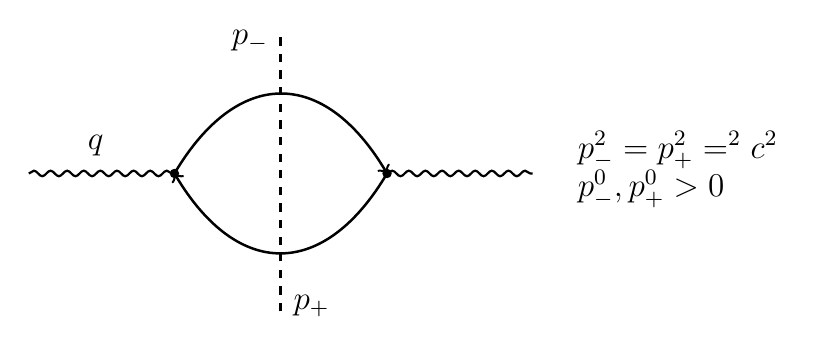
\begin{tikzpicture}[x=1cm,y=1cm,every node/.style={font=\large}]
 \coordinate (L) at (-3.2,0); \coordinate (a) at (-1.35,0);
 \coordinate (b) at (1.35,0); \coordinate (R) at (3.2,0);
 \draw[decorate,decoration={snake,amplitude=1.0pt,segment length=6pt},line width=.8pt] (L)--(a);
 \draw[decorate,decoration={snake,amplitude=1.0pt,segment length=6pt},line width=.8pt] (b)--(R);
 \draw[->,line width=.9pt] (a) .. controls (-.55,1.35) and (.55,1.35) .. (b);
 \draw[->,line width=.9pt] (b) .. controls (.55,-1.35) and (-.55,-1.35) .. (a);
 \fill (a) circle (1.7pt); \fill (b) circle (1.7pt);
 \draw[dashed,line width=1.05pt] (0,-1.75)--(0,1.75);
 \node at (-2.35,.35) {$q$};
 \node[anchor=south east,fill=white,inner sep=1pt] at (-.12,1.50) {$p_-$};
 \node[anchor=north west,fill=white,inner sep=1pt] at (.12,-1.50) {$p_+$};
 \node[align=left,right] at (3.65,.05) {$p_-^2=p_+^2=\me^2c^2$\\$p_-^0,p_+^0>0$};
\end{tikzpicture}

 \caption{QED 真空极化的 $e^-e^+$ 幺正性割线。虚线割线把费米子圈的两条内部线同时置于正能质量壳；其相空间阈值 $s=4\me^2c^2$ 产生 $\Pi_R(s)$ 的分支点。}
 \label{fig:qed-vacpol-cut-dp9}
\end{figure}

\begin{figure}[htbp]
 \centering
 
\includegraphics[width=0.82\textwidth]{qed_vacpol_dispersion_dp9.png}
 \caption{同一个重整化后的真空-极化函数的两种独立计算。实线直接数值积分 \eqnrefs{eq:Pi-spacelike-r12}；虚线只使用类时 $e^-e^+$ 谱权重 \eqnrefs{eq:qed-vacpol-spectral-weight-dp9} 代入色散关系 \eqnrefs{eq:qed-vacpol-dispersion-dp9}。两者重合验证了割线 $\to$ 色散的闭合链。}
 \label{fig:qed-vacpol-dispersion-dp9}
\end{figure}

这同时解释了自能与 LSZ 的关系，但需要区分三个容易混在一起的量：裸场与重整化场之间的场重整化常数 $Z_2$、某一给定场变量的精确二点函数极点留数，以及在壳方案中人为选成单位值的重整化传播子留数。它们彼此相关，却不是同一个定义。

先保留红外调节参数，使带电粒子的极点与连续谱割线暂时分离。对任意固定未来指向单位类时方向 $u^\mu$，沿 $p^\mu=\lambda u^\mu$ 定义正能投影后的标量逆传播子
\begin{equation*}
 d_+(\lambda)
 =\lambda-\me c-\sigma(\lambda),
\end{equation*}
其中 $\sigma(\lambda)$ 是上一节已经定义的正能投影自能本征值。若物理极点位于 $\lambda=\lambda_*$，则
\begin{equation*}
 d_+(\lambda_*)=0.
\end{equation*}
在简单极点条件 $d_+'(\lambda_*)\neq0$ 下，Laurent 展开给
\begin{equation}
 \boxed{
 Z_{\rm pole}
 =\frac{1}{d_+'(\lambda_*)}
 =\frac{1}{1-\sigma'(\lambda_*)}.}
 \label{eq:qed-pole-residue-selfenergy-dp9}
\end{equation}
这里 $Z_{\rm pole}$ 是“当前所用场变量的精确二点函数留数”，它才是谱表示中单粒子极点的权重。若采用一般重整化方案，LSZ 外腿因子由这个物理极点留数补偿；若采用在壳方案，则通过场强反项选择重整化场，使
\begin{equation*}
 Z_{\rm pole}^{(R)}=1.
\end{equation*}
这并不意味着裸场与重整化场之间的 $Z_2$ 等于 1。相反，$Z_2$ 正是反项参数的一部分，它被调节来使重整化后的传播子满足单位留数条件。因而“$Z_2$”“LSZ 极点留数”和“在壳归一化后的单位留数”必须在叙述中分开。

从谱论角度看，自能首先移动并重塑精确二点函数的单粒子极点；LSZ 随后取这个极点的留数并截去外腿传播子。圈自能对散射振幅的外腿影响因此通过极点位置与极点留数进入，而不是通过一个未定义的“$\partial/\partial\slashed p$”直接进入。

\begin{note}[无质量 QED 与 LSZ]
严格的无质量 QED 中，带电粒子总伴随任意软光子云；在非微扰谱意义上，由局域带电场产生的带电扇区具有红外粒子（infraparticle）结构，因此教科书式的孤立单粒子极点与 LSZ 约化需要红外调节参数、Bloch--Nordsieck/KLN 包容可观测量，或经过软光子缀饰的渐近态才能严格闭合。树级与固定阶在壳 QED 公式按受控的红外调节程序理解：先用调节器把单粒子极点与连续谱分开，从而分别定义受调节的极点权重 $Z_{\rm pole}^{(e)}$、场重整化常数 $Z_2$ 与散射振幅；随后在包容可观测量或缀饰态振幅中消去调节器依赖。这个红外问题不改变有质量电子的 Wigner 自旋分类，但会改变“局域带电场与精确渐近单粒子极点”之间最朴素的一一对应。
\end{note}

QED 一圈层与一般 QFT 的谱结构逐项对应：真空极化的 $e^-e^+$ 割线给出谱密度，色散关系由它重建类空区的实部；电子自能的割线决定连续谱阈值，而极点邻域导数首先决定当前场变量的 $Z_{\rm pole}^{(e)}$；在壳条件再据此固定场重整化常数 $Z_2$，LSZ 则用相应极点权重完成外腿归一化；交叉关系则把同一个截肢核连接到 Compton 散射、湮灭与对产生的不同物理区。新的圈图形状因子均应沿“极点与割线位置 $\to$ 不连续度 $\to$ 减法与重整化 $\to$ 物理投影”的顺序组织。

